\documentclass{beamer}
\usetheme{Madrid}
\usepackage[T1]{fontenc}
\usepackage{mathpazo}
\usepackage{graphicx}
\usepackage{booktabs}
\usepackage{tikz}
\usetikzlibrary{positioning,arrows.meta,shapes.geometric,fit,backgrounds,calc}
\definecolor{cetnavy}{RGB}{10,26,63}
\definecolor{cetlight}{RGB}{225,231,242}
\setbeamercolor{structure}{fg=cetnavy}
\setbeamercolor{frametitle}{bg=cetnavy,fg=white}
\setbeamercolor{title}{bg=cetnavy,fg=white}
\setbeamertemplate{navigation symbols}{}
% =====================================================================
%  EDIT YOUR DETAILS HERE — this ONE file feeds every abstract & deck.
%  (Change a value, recompile; all 36 documents update.)
% =====================================================================
\newcommand{\seminarName}{Aflah Muhammed P}      % <-- your full name (guessed from your email; please verify)
\newcommand{\seminarRoll}{TVE00CS000}            % <-- your university register/roll number
\newcommand{\seminarClassRoll}{00}               % <-- your class roll no (the short one)
\newcommand{\seminarGuide}{Prof.\ <Guide Name>}  % <-- your guide
\newcommand{\seminarDept}{Department of Computer Science and Engineering}
\newcommand{\seminarCollege}{College of Engineering Trivandrum}
\newcommand{\seminarShortCollege}{CET}           % shown in the slide footer, e.g. "Aflah Muhammed P (CET)"
\newcommand{\seminarShortTitle}{B.Tech Seminar}  % middle of the slide footer
\newcommand{\seminarDate}{July 31, 2026}
% ---------------------------------------------------------------------
% Optional: put a logo image named  cet_logo.png  in this folder and it
% will appear on every title slide automatically. If absent, it is skipped.
% =====================================================================

\title[\seminarShortTitle]{Agentic Retrieval-Augmented Generation: A Survey}
\author[\seminarName\ (\seminarShortCollege)]{\seminarName \\ \seminarRoll \\ Roll No: \seminarClassRoll \\ Guide: \seminarGuide}
\institute[\seminarShortCollege]{\seminarDept \\ \seminarCollege}
\date{\seminarDate}
\titlegraphic{\IfFileExists{cet_logo.png}{\includegraphics[height=1.1cm]{cet_logo.png}}{}}
\begin{document}
\begin{frame}\titlepage\end{frame}
\begin{frame}{Table of Contents}\tableofcontents\end{frame}
\section{Introduction}
\begin{frame}{What is Agentic RAG?}
\textbf{\textit{From static retrieval to autonomous reasoning}}
\begin{itemize}
\item LLMs are powerful but limited by static training data.
\item RAG grounds answers in retrieved external evidence.
\item Traditional RAG uses fixed, single-shot pipelines.
\item Agentic RAG embeds autonomous agents into the pipeline.
\item Agents plan, retrieve, reflect, and adapt dynamically.
\end{itemize}
\end{frame}

\begin{frame}{Scope of this Survey}
\begin{itemize}
\item Authors: Singh, Ehtesham, Kumar, Talaei Khoei, Vasilakos.
\item Published as arXiv:2501.09136, 2025.
\item Defines four agentic design patterns.
\item Proposes a taxonomy of RAG architectures.
\item Reviews frameworks, benchmarks, and applications.
\end{itemize}
\end{frame}

\section{Literature Survey}
\begin{frame}{Evolution of RAG Paradigms}
\begin{itemize}
\item \textbf{\textit{Na\"ive RAG:}} retrieve-then-generate, keyword based.
\item \textbf{\textit{Advanced RAG:}} re-ranking, query rewriting, dense retrieval.
\item \textbf{\textit{Modular RAG:}} composable, reconfigurable components.
\item \textbf{\textit{Graph RAG:}} structured relational knowledge retrieval.
\item \textbf{\textit{Agentic RAG:}} autonomous, adaptive, multi-step control.
\end{itemize}
\end{frame}

\begin{frame}{Foundations Built Upon}
\begin{itemize}
\item Lewis et al. (2020): original RAG formulation.
\item Self-RAG: self-reflective retrieval and critique.
\item Corrective RAG: retrieval-quality feedback loops.
\item Agent frameworks: ReAct, planning, tool use.
\end{itemize}
\end{frame}

\section{Motivation}
\begin{frame}{Why Agents in RAG?}
\begin{itemize}
\item Static pipelines retrieve once, cannot self-correct.
\item Complex queries need multi-step, iterative reasoning.
\item Real tasks span multiple heterogeneous data sources.
\item Retrieval strategy should adapt to query complexity.
\item Autonomy enables synthesis, verification, and orchestration.
\end{itemize}
\end{frame}

\section{Problem Statement}
\begin{frame}{The Gap Addressed}
\begin{itemize}
\item Traditional RAG lacks adaptability and reasoning depth.
\item No mechanism to judge retrieval sufficiency.
\item Poor handling of multi-hop, cross-source questions.
\item The field lacks a unifying organizing framework.
\item Need: a taxonomy of agentic RAG designs.
\end{itemize}
\end{frame}

\section{Objectives}
\begin{frame}{Goals of the Survey}
\begin{itemize}
\item Formalize the four agentic design patterns.
\item Propose a principled taxonomy of architectures.
\item Contrast agentic RAG with na\"ive and advanced RAG.
\item Compile tasks, datasets, and evaluation benchmarks.
\item Map applications and open research challenges.
\end{itemize}
\end{frame}

\section{Methodology Overview}
\begin{frame}{The Agentic RAG Loop}
\begin{center}
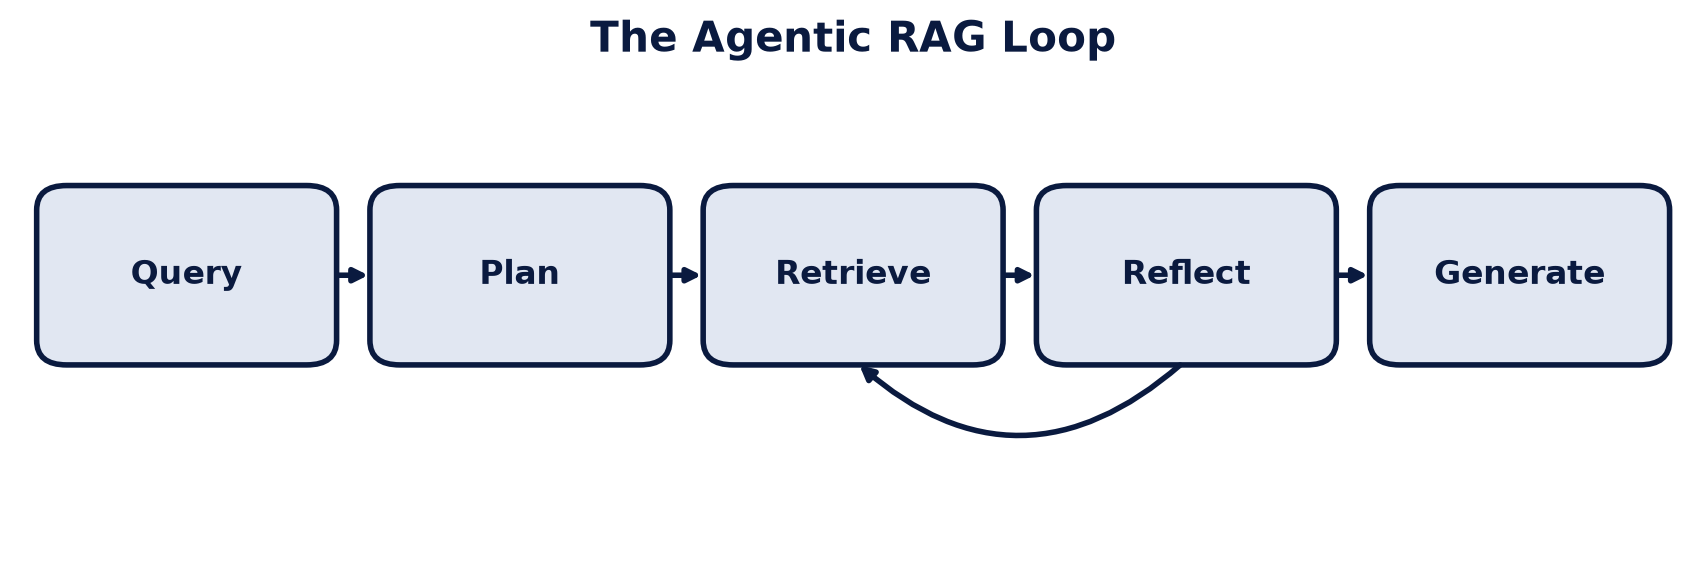
\includegraphics[width=0.9\textwidth,height=0.62\textheight,keepaspectratio]{images/agenticrag_1.png}
\end{center}
\begin{itemize}
\item Reflection loop revisits retrieval until sufficient.
\item Planning decomposes queries into subtasks.
\end{itemize}
\end{frame}

\begin{frame}{Four Agentic Design Patterns}
\begin{itemize}
\item \textbf{\textit{Reflection:}} self-evaluate and refine outputs.
\item \textbf{\textit{Planning:}} decompose tasks into ordered subtasks.
\item \textbf{\textit{Tool use:}} call APIs, search, and calculators.
\item \textbf{\textit{Multi-agent:}} collaborate and specialize in parallel.
\end{itemize}
\end{frame}

\section{System Architecture}
\begin{frame}{Layered Agentic RAG Stack}
\begin{center}
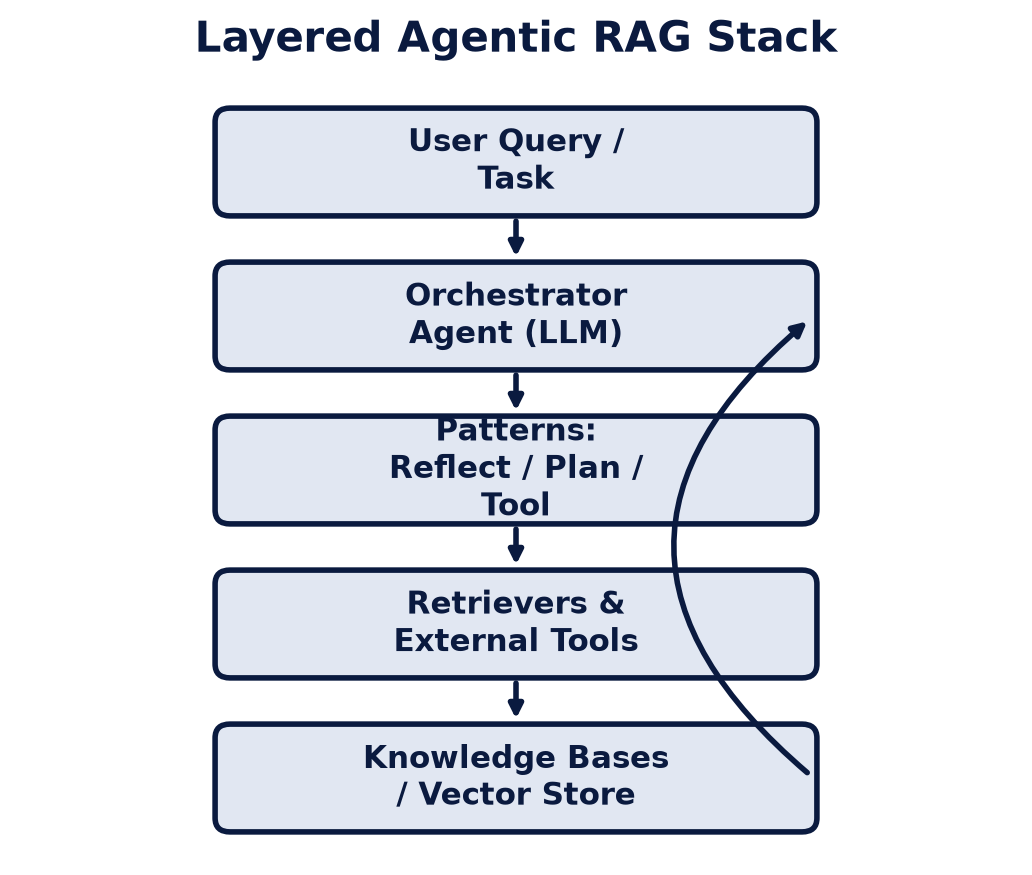
\includegraphics[width=0.9\textwidth,height=0.62\textheight,keepaspectratio]{images/agenticrag_2.png}
\end{center}
\end{frame}

\section{Data Collection}
\begin{frame}{Survey Scope and Sources}
\textbf{\textit{Taxonomy dimensions}}
\begin{itemize}
\item Agent cardinality: single vs. multiple agents.
\item Control structure: sequential, hierarchical, collaborative.
\item Autonomy: degree of independent decision-making.
\item Knowledge representation: flat vs. graph-structured.
\end{itemize}
\end{frame}

\begin{frame}{Benchmarks and Tools Catalogued}
\textbf{\textit{Evaluation resources}}
\begin{itemize}
\item Retrieval: BEIR, MS MARCO, TREC-DL.
\item Multi-hop QA: HotpotQA, MuSiQue, 2WikiMultihopQA.
\item RAG-specific: RAGBench (TRACe), BERGEN, FlashRAG.
\end{itemize}
\textbf{\textit{Frameworks}}
\begin{itemize}
\item LangGraph, LlamaIndex, CrewAI, AG2, OpenAI Swarm.
\end{itemize}
\end{frame}

\section{Model Development}
\begin{frame}{Taxonomy of Agentic RAG Architectures}
\begin{itemize}
\item \textbf{\textit{Single-agent (router):}} centralized retrieval routing.
\item \textbf{\textit{Multi-agent:}} specialized agents, parallel sources.
\item \textbf{\textit{Hierarchical:}} tiered strategic oversight.
\item \textbf{\textit{Corrective:}} feedback-driven self-correction.
\item \textbf{\textit{Graph-based:}} Agent-G, GeAR relational retrieval.
\item \textbf{\textit{Document workflows (ADW):}} end-to-end automation.
\end{itemize}
\end{frame}

\begin{frame}{Adaptive Agentic RAG Routing}
\begin{center}
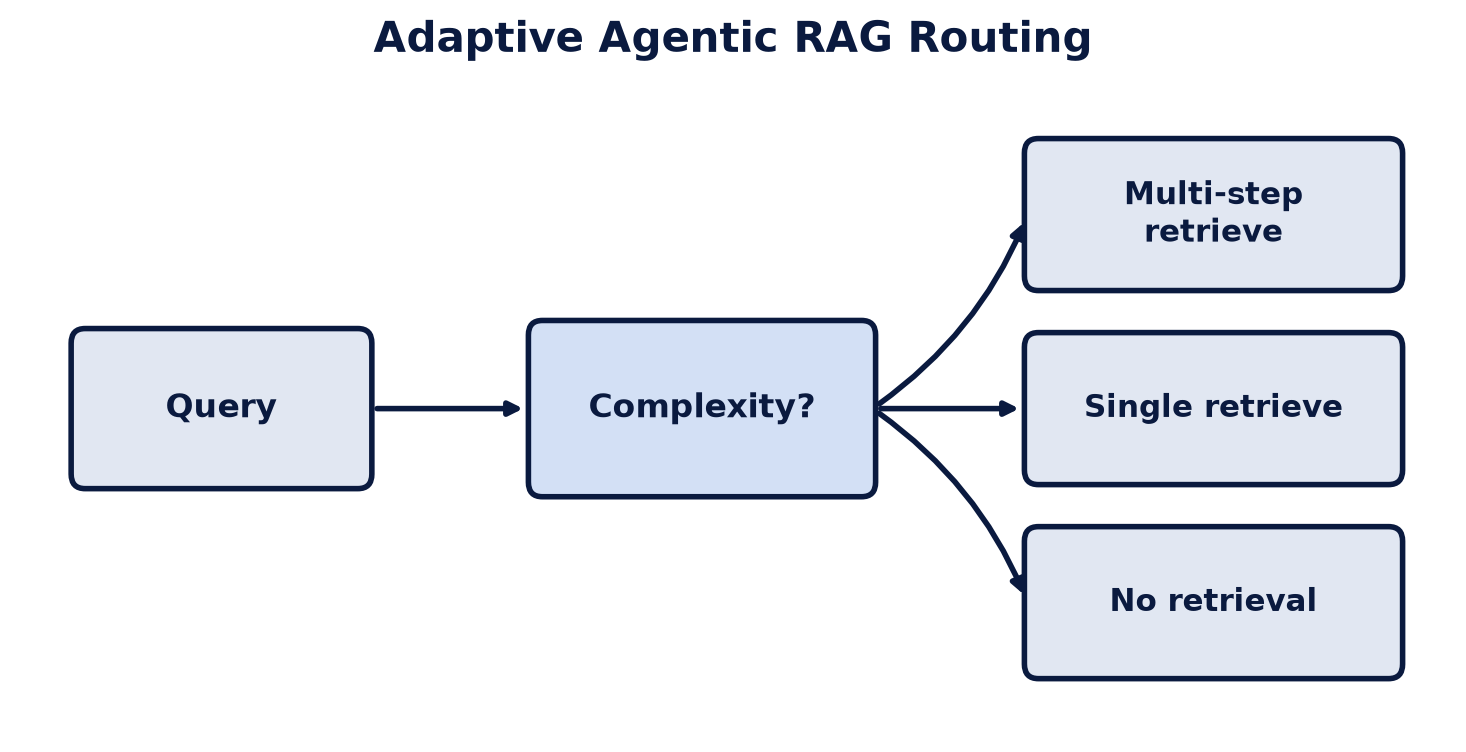
\includegraphics[width=0.9\textwidth,height=0.62\textheight,keepaspectratio]{images/agenticrag_3.png}
\end{center}
\begin{itemize}
\item A classifier routes by estimated query difficulty.
\item Balances answer quality against retrieval cost.
\end{itemize}
\end{frame}

\section{Results}
\begin{frame}{Comparing RAG Paradigms}
\begin{center}
\begin{tabular}{@{}lccc@{}}
\toprule
Paradigm & Adaptivity & Multi-step & Multi-agent \\
\midrule
Na\"ive RAG & Low & No & No \\
Advanced RAG & Medium & Limited & No \\
Modular RAG & Medium & Some & No \\
Agentic RAG & High & Yes & Yes \\
\bottomrule
\end{tabular}
\end{center}
\begin{itemize}
\item Agentic designs add reflection and dynamic control.
\item Gains come with higher orchestration overhead.
\end{itemize}
\end{frame}

\begin{frame}{Application Domains Surveyed}
\begin{itemize}
\item Healthcare: evidence-grounded clinical support.
\item Finance: analysis over dynamic market data.
\item Education: adaptive tutoring and retrieval.
\item Enterprise: document processing and workflows.
\end{itemize}
\end{frame}

\section{Discussions}
\begin{frame}{Why Agentic RAG Works}
\begin{itemize}
\item Iterative retrieval improves evidence sufficiency.
\item Planning enables robust multi-hop reasoning.
\item Specialization scales across heterogeneous sources.
\item Reflection reduces hallucination and errors.
\item Trade-off: added latency and coordination cost.
\end{itemize}
\end{frame}

\section{Challenges}
\begin{frame}{Open Challenges}
\begin{itemize}
\item Coordinating communication across multiple agents.
\item Scalability and latency at large data volume.
\item Optimal tool selection among many options.
\item Standardized, reliable evaluation methodologies.
\item Memory management, governance, and ethics.
\end{itemize}
\end{frame}

\section{Future Work}
\begin{frame}{Research Directions}
\begin{itemize}
\item Unified benchmarks for agentic RAG evaluation.
\item Efficient coordination and lightweight orchestration.
\item Long-term memory and persistent context.
\item Multimodal and graph-enhanced retrieval.
\item Trustworthy, governable, and safe deployments.
\end{itemize}
\end{frame}

\section{Conclusion}
\begin{frame}{Conclusion}
\begin{itemize}
\item Agentic RAG augments retrieval with autonomous agents.
\item Four patterns: reflection, planning, tool use, collaboration.
\item Survey offers a taxonomy of seven architectures.
\item Enables adaptive, multi-step, cross-source reasoning.
\item Coordination, evaluation, and governance remain open.
\end{itemize}
\end{frame}

\section{References}
\begin{frame}{References}
\footnotesize
\begin{itemize}
\item A. Singh, A. Ehtesham, S. Kumar, T. Talaei Khoei, and A. V. Vasilakos, ``Agentic Retrieval-Augmented Generation: A Survey on Agentic RAG,'' arXiv:2501.09136, 2025.
\item P. Lewis et al., ``Retrieval-Augmented Generation for Knowledge-Intensive NLP Tasks,'' in Proc. NeurIPS, 2020.
\item A. Asai, Z. Wu, Y. Wang, A. Sil, and H. Hajishirzi, ``Self-RAG: Learning to Retrieve, Generate, and Critique through Self-Reflection,'' in Proc. ICLR, 2024.
\end{itemize}
\end{frame}
\begin{frame}\vfill\centering{\Huge Thank You}\vfill\end{frame}
\end{document}
